%!TEX root = ../thesis.tex
%*******************************************************************************
%*********************************** Second Chapter *****************************
%*******************************************************************************

\chapter{Statistical aspects of the epigenetic clock}  

\ifpdf
\graphicspath{{Chapter2/Figs/pdf/}}
\else
\graphicspath{{Chapter2/Figs/svg/}}
\fi


\section{Analysing the blood methylome to study human ageing}

\smallskip

\subsection{Building a DNA methylation dataset from public data}

\smallskip

During the last years large amounts of DNA methylation data have been generated to study complex diseases and ageing \cite{Rakyan2011,Flanagan2015}. Many of these datasets can be obtained from public repositories, such as the NCBI-hosted Gene Expression Omnibus (\acrshort{GEO}) \cite{Edgar2002}. Given its clinical accessibility and ease of collection, blood is one of the most commonly profiled tissues in human DNA methylation studies \cite{Flanagan2015}, including published studies on developmental disorders \cite{Aref-Eshghi2018} (see Chapter 3). Therefore, I decided to use blood as my surrogate tissue to broaden our understanding of the human epigenetic ageing clock.

\bigskip

Furthermore, most of these human datasets have been generated using different versions of the Illumina Infinium array technology, with the Illumina Infinium HumanMethylation450 array (450K) being the most frequently used platform \cite{Flanagan2015}. Additionally, given that the different array versions have different chemistries and biases \cite{Bibikova2009,Bibikova2011,Pidsley2016}, I decided to focus on 450K data for my analyses. Using the \textit{GEOquery} R package \cite{Davis2007}, I programmatically downloaded from GEO all the DNA methylation data that I could find or human blood that satisfied the following criteria:

\begin{itemize}
	
	\item Raw DNA methylation data was available (i.e. IDAT files). This was required so the pre-processing pipeline and the batch effect correction (which requires access to control probes intensities, see `xxxxxxx' section) could be consistently applied across all the samples in the study.
	
	\item Metadata for the samples was available, with the chronological age as an absolute requirement. 
	
	\item In order to study physiological ageing, the blood samples corresponded to humans without any major disease. However, it is important to mention that I could never be completely certain of this, since there could be a lack of diagnosis and/or lack of reporting of the disease in the metadata. 
	
\end{itemize}

\smallskip

This allowed me to assembly a human blood DNA methylation dataset for healthy individuals (after \acrshort{QC}, total $N=2218$) with the characteristics shown in Table~\ref{table:c2_table1}, which spans the entire human lifespan (0.5 to 101 years). Fig.~\ref{fig:c2_fig1} shows that the chronological age distribution is bimodal, with peaks around 10.69 and 58.81 years respectively. This reflects a sampling bias in human population studies, with more data being generated for the periods of postnatal development and during the appearance of age-related disease. However, in order to understand the development of complex diseases as a consequence of the ageing process, efforts should be made to sample people also in their middle ages, before the diseases are normally diagnosed.   


\begin{table}
%\centering
\small
	\begin{tabular}{ p{2cm} p{1cm} p{1cm} p{1cm} p{2cm} p{6cm} }
		\toprule
		\textbf{Batch name} & \textbf{N$_{\female}$} & \textbf{N$_{\male}$} & \textbf{N} & \textbf{Median age (years)} & \textbf{Other comments} \\
		\midrule
		Europe & 0 & 121 & 121 & 10.96 & - \\
		Feb\_2016 & 0 & 1 & 1 & 0.50 & - \\
		GSE104812 & 19 & 29 & 48 & 9.00 & - \\
		GSE111629 & 111 & 124 & 235 &  71.00 & - \\
		GSE40279 & 336 & 314 & 650 & 65.00 & - \\
		GSE41273 & 0 & 51 & 51 & 10.25 & - \\
		GSE42861 & 239 & 96 & 335 & 55.00 & - \\
		GSE51032 & 253 & 78 & 331 & 54.57 & Only people that remained cancer-free in the follow-up after sample collection were included  \\
		GSE55491 & 1 & 5 & 6 & 29.50 & - \\
		GSE59065 & 49 & 46 & 95 & 34.00 & - \\
		GSE61496 & 72 & 78 & 150 & 57.00 & Only one member of each twins pair was included \\
		GSE74432 & 29 & 22 & 51 & 12.00 & - \\
		GSE81961 & 25 & 0 & 25 & 30.05 & - \\
		GSE97362 & 39 & 80 & 119 & 13.00 & - \\
		\midrule
		\textbf{Total} & 1173 & 1045 & 2218 & 55.00 & - \\ 
		\bottomrule
	\end{tabular}
	\vspace*{3mm}
	\caption[Overview of the blood DNA methylation dataset from healthy individuals]{Overview of the blood DNA methylation dataset from healthy individuals. All the batches were downloaded from GEO \cite{Edgar2002}, with the exception of `Europe' and `Feb\_2016', which were generated in-house by our collaborators in Canada (see Chapter 3). $N_{\female}$: number of samples from females. $N_{\male}$: number of samples from males. $N$: total number of samples. These numbers correspond to the samples left after applying quality control (QC, see `Overview of the DNA methylation pre-processing pipeline')}
	\label{table:c2_table1}
\end{table} 


\begin{figure}[htbp!] 
	\centering    
	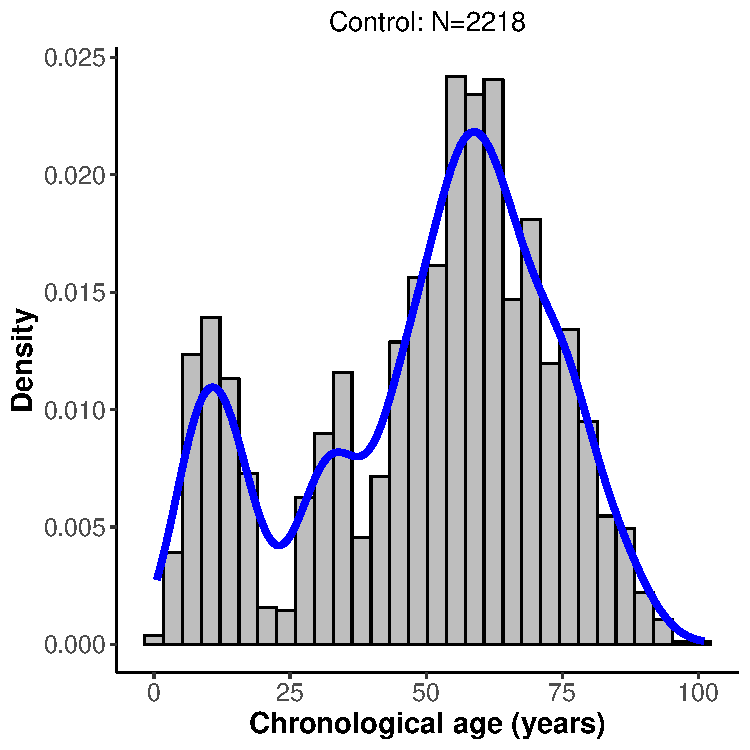
\includegraphics[width=0.6\textwidth]{C2_Fig1}
	\vspace*{2mm}
	\caption[Chronological age distribution in our healthy individuals]{Chronological age distribution in our healthy individuals. Histogram showing the chronological age distribution for all the healthy individuals included in our DNA methylation dataset. The blue line represents the 1D kernel density estimate, as calculate by the \textit{stat\_density} function in R with default parameters.}
	\label{fig:c2_fig1}
\end{figure}

\smallskip

\subsection{Main DNA methylation data pre-processing pipeline}

\smallskip

The analysis of DNA methylation data generated in Illumina arrays has been a topic of huge discussion and statistical innovation in the epigenetic community. There are plenty of reviews in the literature that discuss the different steps that should be involved in the pre-processing of this data type \cite{Wilhelm-Benartzi2013,Morris2015,Liu2016}. More specifically, a recent study by Je Liu and Kimberly D. Siegmund systematically benchmarked the pre-processing methods available for the 450K array in order to reduce variation among technical replicates and improve the detection of biological differences \cite{Liu2016}. Inspired by their results, I implemented, using the \textit{minfi} R package \cite{Aryee2014}, a pre-processing pipeline for the 450K data with the following steps (Fig.~\ref{fig:c2_fig2}):

\begin{enumerate}
	
	
	\item \textbf{Background correction}. I used the \textit{noob} method \cite{TricheJr2013}, as implemented in the \textit{preprocessNoob} function from the \textit{minfi} R package \cite{Aryee2014}. \textit{noob} allows accounting for technical variation in the background (i.e. non-specific) fluorescence signal, which can lead to a reduced dynamic range for the $\beta$-values obtained (Fig.~\ref{fig:c2_fig2}b, Fig.~\ref{fig:sc2_fig1}) \cite{TricheJr2013}. Briefly, when measuring fluorescence intensities in the Illumina array platforms, the observed intensity (also known as foreground, $X_f$) is composed of:
	
	\begin{align}
	X_f = X_s + X_b
	\end{align}
	
	where $X_s$ is the true signal and $X_b$ is the background signal. Making use of a normal-exponential convolution (which assumes $X_b\sim N(\mu, \sigma^2)$ and $X_s\sim Exp(\gamma)$) and the `out-of-band' (\acrshort{OOB}) intensities (fluorescence signals in the opposite colour channel in Infinium I probes) to model $X_b$ , \textit{noob} is capable of estimating $X_s$ given $X_f$. Furthermore, I also applied the default dye-bias correction strategy, which controls for the different average intensities in the two colour channels \cite{TricheJr2013}. 
	
		\item \textbf{Quality control} (QC). Following guidelines from the \textit{minfi} R package \cite{Aryee2014}, I kept only those samples that satisfied the following criteria:
		
		\begin{enumerate}
			
			\item The sex predicted from the DNA methylation data (\acrshort{Sexp}) was the same as the reported sex in the metadata. The sex was predicted  using the \textit{getSex} function from the \textit{minfi} R package \cite{Aryee2014}, which employs intensity information from the sex chromosomes, such that:
			
			\begin{align}
			\text{Sex}_{p} = 
			\begin{cases}
			\text{female, } &\text{if: } (\mathrm{median}\left\{\log_2(M_{y}+U_{y})\right\} -  \mathrm{median}\left\{\log_2(M_{x}+U_{x})\right\}) < c \\
			\text{male, } &\text{if: } (\mathrm{median}\left\{\log_2(M_{y}+U_{y})\right\} -  \mathrm{median}\left\{\log_2(M_{x}+U_{x})\right\}) \geq c \\
			\end{cases}
			\end{align}
			
			where $M_{y}$ and $U_{y}$ represent the methylated and unmethylated intensity measurements for the array probes in the Y chromosome, $M_{x}$ and $U_{x}$ represent the methylated and unmethylated intensity measurements for the array probes in the X chromosome and $c$ is a predefined cutoff (default in \textit{minfi}: $c=-2$).
			
			\smallskip
			
			\item They were not outliers according to their global intensity values after background correction, such that:
			
			\begin{align}
			\frac{\mathrm{median}\left\{\log_2(M_{i})\right\} + \mathrm{median}\left\{\log_2(U_{i})\right\}}{2} \geq 10.5
			\end{align}
			
			where $M_{i}$ and $U_{i}$ represent the background-corrected methylated and unmethylated intensity measurements for all the 450K array probes (Fig.~\ref{fig:sc2_fig2}).
			
		\end{enumerate} 
	
	\item \textbf{Probe filtering}. I filtered out the following types of probes:
	
	\begin{itemize}
		
		\item Probes that contain \acrshort{SNP}s at the single base extension site (position 0) or at the proximal CpG on the probe (positions 1-2), using the \textit{dropLociWithSnps} function in the \textit{minfi} package \cite{Aryee2014}. 
		
		\item Cross-reactive probes, as defined by Chen \textit{et al.} \cite{Chen2013}. These are probes that can co-hybridise to alternative genomic sequences that are highly homologous to the target sequences \cite{Chen2013}.  
		
		\item  Probes that map to the sex chromosomes (X and Y).
	
	\end{itemize}
	
	It is important to mention that other authors have also filtered out probes with high detection p-value or low bead counts across samples \cite{Wilhelm-Benartzi2013,Morris2015}. However, I did not include these filters since it was not pointed out in the \textit{minfi} guidelines \cite{Aryee2014,Fortin2015} and it could complicate further downstream analyses (e.g. different sets of probes missing across different batches, discarding probes that were needed for cell composition estimation, ...).     
	
	
	\begin{figure}[htbp!] 
		\centering    
		\includegraphics[width=0.8\textwidth]{C2_Fig2}
		\vspace*{2mm}
		\caption[Main DNA methylation data pre-processing pipeline]{Main DNA methylation data pre-processing pipeline. \textbf{a.} Flowchart showing the main steps that I implemented to pre-process the DNA methylation data for the healthy individuals. The number of samples (N$_{samples}$) and the number of array probes (N$_{probes}$) left after each step are also specified. \textbf{b.}  $\beta$-value distributions, calculated using the raw fluorescence intensities (i.e. before any pre-processing), for the samples in the GSE41273 batch. Each curve represents a different sample. In grey: 51 samples that passed quality control (QC). In red: 2 samples that failed QC.  \textbf{c.} As in b., but calculating the $\beta$-values after background correction. \textbf{d.} As in b., but calculating the $\beta$-values after background correction, QC, probe filtering and BMIQ normalisation (i.e. the final $\beta$-values that I used for downstream analyses). Note that the samples that failed QC have been removed.}
		\label{fig:c2_fig2}
	\end{figure}
	
	
	\item \textbf{$\beta$-value calculation}. The methylation status of a given CpG site in one of the array probes is normally quantified using the $\beta$-value statistic ($\beta$), which can be calculated as \cite{Wilhelm-Benartzi2013,Du2010}:
	
	\begin{align}
	\beta_i = \frac{\text{max}(M_i,0)}{\text{max}(M_i,0) + \text{max}(U_i,0) + \alpha}
	\end{align}
	
	where $M_i$ and $U_i$ represent the methylated and unmethylated intensity measurements for the $i$th-probe and $\alpha$ is a constant offset (in this work $\alpha = 100$, as recommended by Illumina) \cite{Du2010}. 
	
	In a DNA copy (allele) of a single cell, a specific CpG site is either unmethylated or methylated (categorical / binary variable). However, given that a bulk DNA sample from a tissue is composed of thousands of cells (which can include different cell types with different methylation patterns), $\beta$-values result in a continuous variable between 0 and 1. A value of 0 means that all the measured DNA molecules are unmethylated ($0\%$) and a value of 1 means that all the measured DNA molecules are methylated ($100\%$), which is roughly equivalent to say that 100\% of the cells are either unmethylated or methylated respectively in that CpG site for the sampled tissue. The $\beta$-values for a given sample normally follow a bimodal distribution, where the two peaks are centred around 0 and 1 (Fig.~\ref{fig:c2_fig2}d). 
	
	Other authors have used M-values to quantify methylation levels in arrays (Fig.~\ref{fig:sc2_fig3}), which can be calculated as:
	
	\begin{align}
	\text{M-value}_i = \log_2 \left(\frac{\text{max}(M_i,0) + \alpha}{\text{max}(U_i,0) + \alpha}\right)
	\end{align}
	
	with a default offset value of $\alpha=1$.  Du \textit{et al.} reported that $\beta$-values suffer from severe heteroscedasticity for highly methylated or unmethylated CpG sites and therefore the M-values have more desirable statistical properties \cite{Du2010}. However, Zhuang \textit{et al.} later showed that this only becomes a problem in studies with small sample sizes \cite{Zhuang2012} (which is not the case for my analyses). Furthermore, $\beta$-values are easier to interpret biologically and can be readily used in the context of BMIQ normalisation (see below). For these reasons, I choose $\beta$-values as the main methylation variable for this work.
	
	\item \textbf{Beta-mixture quantile normalisation} (\acrshort{BMIQ}). As mentioned in Chapter 1, in the case of the 450K arrays two types of probes / chemistry coexist in the same platform. Infinium I probes and Infinium II probes have different $\beta$-values distributions (a.k.a. Infinium II probe bias). BMIQ is an intra-array normalisation strategy that allows to correct for this bias and has been shown to outperform other methods used in this context \cite{Teschendorff2012,Dedeurwaerder2011,Touleimat2012,Maksimovic2012}. BMIQ fits a three-state beta-mixture model to Infinium I and Infinium II probes separately and then maps the Infinium II probes distribution into the Infinium I probe distribution (Fig.~\ref{fig:c2_fig3}). In the case of unmethylated ($\beta$-values close to 0) and methylated ($\beta$-values close to 1) probes, this is done by transforming probabilities into quantiles. In the case of `hemimethylated' probes (intermediate $\beta$-values), a dilation transformation is applied to preserve the monotonicity and continuity of the data \cite{Teschendorff2012}. I applied BMIQ to my samples and discarded those that failed the normalisation step.  
	
\end{enumerate}

\bigskip
 
\begin{figure}[htbp!] 
	\centering    
	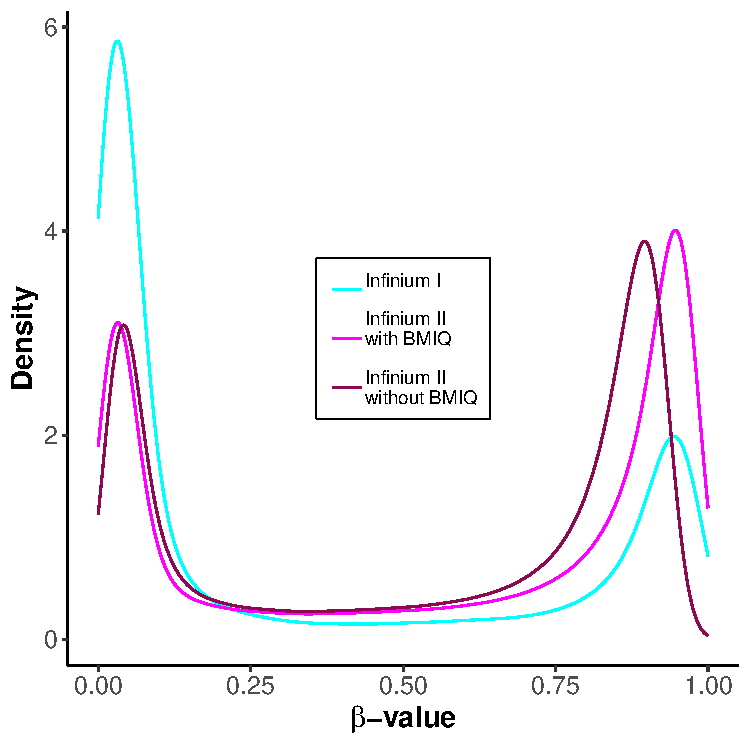
\includegraphics[width=0.8\textwidth]{C2_Fig3}
	\caption[Effect of BMIQ normalisation on the $\beta$-value distribution]{Effect of BMIQ normalisation on the $\beta$-value distribution. The $\beta$-value distributions for different subsets of array probes in a DNA methylation sample from the GSE41273 batch. It can be appreciated how BMIQ transforms the distribution of the Infinium II probes into a distribution more similar to the Infinium I probes.}
	\label{fig:c2_fig3}
\end{figure}

 





\smallskip

\section{Behaviour of Horvath's epigenetic clock during ageing}

\smallskip


\smallskip

\section{Behaviour of other epigenetic clocks during ageing}

\smallskip



\section{Additional methods}

\subsection*{Experimental procedures for DNA methylation data generation}


